\section{Gehäuse}
\label{app:Gehause}
Mit der Software SolidWorks wurde ein Gehäuse für die Platine erstellt. Diese wurde anschließend mit einem 3D-Drucker aus Polylactide (PLA) ausgedruckt.
\begin{figure}[H]
\centering
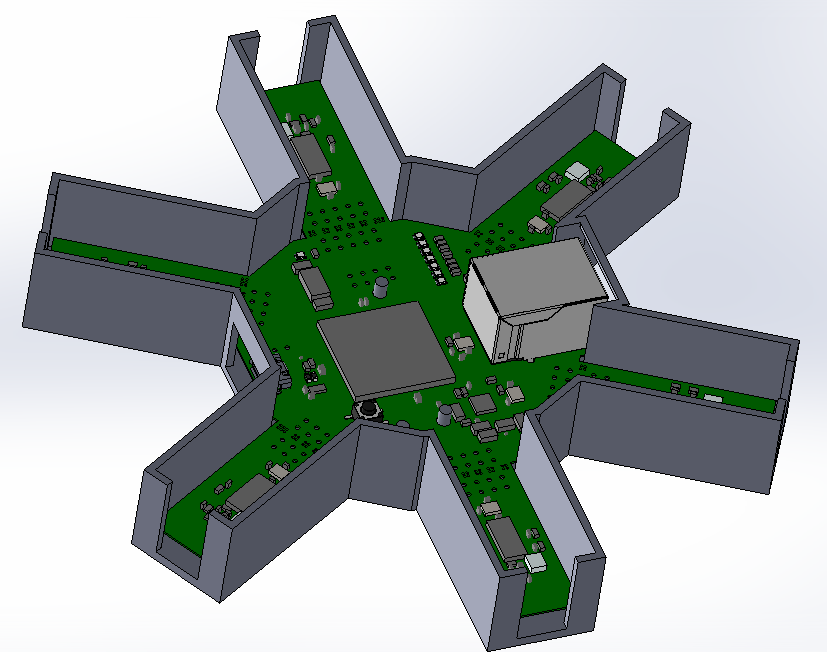
\includegraphics[width=\linewidth]{Abbildungen/Aufnahmen/Bilder/SolidWorks/BoxBildschirmSW}
\caption{Erstellte Box zum Schutz der Basisstation in der Software SolidWorks}
\label{fig:boxbildschirmsw}
\end{figure}




